% !TeX root = skripta-konstitutivni-vztahy.tex
% !TeX lastmodified = 2019-12-11

% TODO Sjednotit creep a tečení

\subsection{Model Norton}\label{sec:norton}
Tento model\footnote{Norton, F. H. "The Creep of Steel at High Temperature", McGraw-Hill, 1929} popisuje sekundární tečení kovů na základě jejich visko-plastického chování, do něhož zahrnuje závislost na teplotě.
Jeho rychlost creepového přetvoření je popsána rovnicí
\begin{equation}
	\dot{\varepsilon}_\text{cr} = C_1 \sigma^{C_2} \exp\left(-\frac{C_3}{T}\right),
\end{equation}
kde
\begin{description}
	\item[$\sigma$] je ekvivalentní napětí (Misesovo)
	\item[$\dot{\varepsilon}_\text{cr}$]je rychlost ekvivalentního creepového přetvoření
	\item[{$T [K]$}] je absolutní teplota
	\item[{$C_1 [\si{\pascal^{-C_2}\per\second}], C_2 [-], C_3 [\si{\kelvin}]$}] jsou materiálové parametry.
\end{description}

Výstupem modelu není přímo velikost, ale jen rychlost přetvoření.
Abychom dostali přetvoření v~daném okamžiku, je třeba ji ještě integrovat v~čase od výchozího (nedeformovaného) stavu.

\begin{figure}[H]
	\centering
	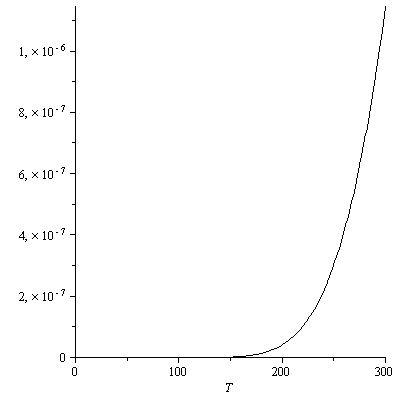
\includegraphics[width=0.3\textwidth]{norton}
	\caption{Závislost rychlosti krípové deformace na teplotě (parametry zvoleny náhodně)}
	\label{fig:model-norton}
\end{figure}
